\section{Testing and verification process}\label{sec:test}
Testing designs before compiling them becomes ever more important as complexity scales. 
In the later stages of the project, a single compilation could take as much as ten minutes, 
highly restricting iterative testing methodologies like divide and conquer\footnote{
    A methodology where debugging statements are printed to console to narrow down the source of a problem.
    Highly reliant on running many test suites in quick succession. 
}. Therefore, the importance of testing via simulations is emphasised. 

To illustrate this process, an example will be outlined. Following an agile-like development methodology 
for this project prioritised producing functional code as quickly as possible. 
For static but repeatable elements, this means a large amount of hardcoded software, 
making the code unwieldy and increasing the difficulty maintaining the codebase.
To improve this, the logic can be synthesised from a FOR loop instead. 

\subsection{The hardcode}
\begin{lstlisting}
initial begin
    colourspace[0] <= 12'hfff;
    colourspace[1] <= 12'hfdf;
    colourspace[2] <= 12'hfbf;
    ... 
    colourspace[7] <= 12'f1f;
    colourspace[8] <= 12'dff;
    ... 
    colourspace[63] <= 12'h11f;
end
\end{lstlisting}
This was generated from the following Python script (modified slightly for clarity):
\begin{lstlisting}[language=Python]
    r = 15
    g = 15
    b = 15
    for count in range(0,64):
        print(f"colorspace[{count}] <= 12'h{r:x}{g:x}{b:x};")
        g = g - 2
        if(g < 0):
            r = r - 2
            g = 15
\end{lstlisting}

\subsection{Rewrite in Verilog}
The hardcoded logic can be synthesised from a FOR loop, written in Verilog directly in this case.
This is almost a direct translation from the Python script to Verilog, however there are a number of differences. 
Since the code does not need to be printed to be copied, that stage is omitted entirely. Instead, the assignment of the 
colour to \lstinline|colourspace| is made directly through an intermediary variable \lstinline|tcol|, 
which is made of the \lstinline|r|, \lstinline|g|, and \lstinline|b| bitshifted to their respective places.
\begin{lstlisting}[language=Verilog]
for(i=0;i<64;i=i+1)begin
    tcol = r<<8;
    tcol = tcol + g<<4;
    tcol = tcol + b;
    colourspace[i] = tcol;
    g = g - 2;
    if(g < 1) begin
        r = r - 2;
        g = 4'hf;
    end
end
\end{lstlisting}
This can then be run in a test bench to see the resultant values of
\lstinline|tcol|, \lstinline|r|, \lstinline|g|, \lstinline|b|, and \lstinline|colourspace|.
\begin{figure}[H]
    \centering
    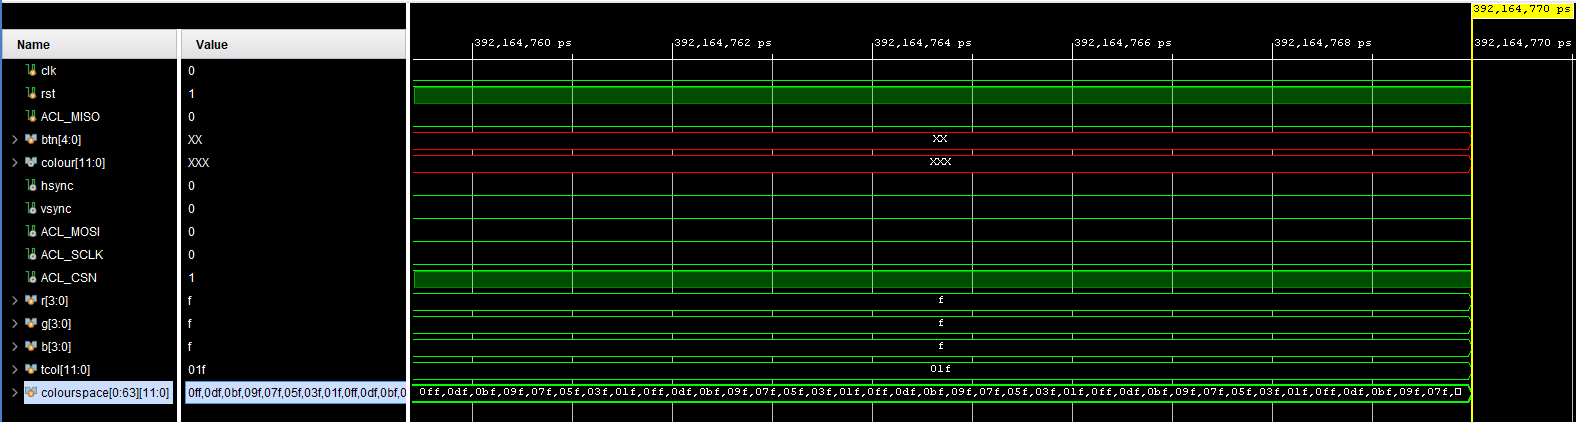
\includegraphics[width=\textwidth]{figures/tb/1.png}
\end{figure}
The resulting colour values are not quite correct, with the red value stuck at 0.

\begin{minipage}{0.475\linewidth}
\begin{lstlisting}[language=Verilog]
for(i=0;i<64;i=i+1)begin
    colourspace[i] = r<<8 + g<<4 + b;
    g = g - 4'h2;
    if(g < 4'h1) begin
        r = r - 4'h2;
        g = 4'hf;
    end
end    
\end{lstlisting}
\end{minipage}\hfill
\begin{minipage}{0.5\linewidth}
    \centering
    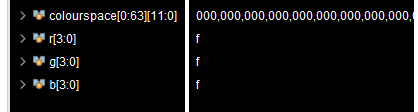
\includegraphics[width=\linewidth]{figures/tb/2.png}
\end{minipage}
This attempts to perform the bit-shift in a single line, however the end result is all 0.
The intermediary variable is necessary. 

\begin{minipage}{0.475\linewidth}
\begin{lstlisting}[language=Verilog]
for(i=0;i<64;i=i+1)begin
    tcol = tcol + g<<4;
    tcol = tcol + b;
    colourspace[i] = tcol;
    g = g - 4'h2;
    if(g < 4'h1) begin
        r = r - 4'h2;
        g = 4'hf;
    end
end
\end{lstlisting}
\end{minipage}\hfill
\begin{minipage}{0.5\linewidth}
    \centering
    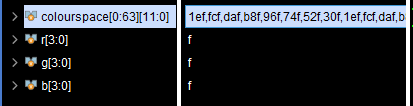
\includegraphics[width=\linewidth]{figures/tb/3.png}
\end{minipage}
This indicates the red bit-shift is always returning 0 and non-functional. 
The gradient produced is also not what is intended. It may be better to move 
to subtracting a constant value. 

\begin{minipage}{0.475\linewidth}
\begin{lstlisting}[language=Verilog]
for(i=0;i<64;i=i+1)begin
    colourspace[i] = tcol;
    tcol = tcol - 12'h020;
    if(tcol[7:4] < 4'h1) begin
        tcol = tcol - 12'h200;
    end
end
\end{lstlisting}
\end{minipage}\hfill
\begin{minipage}{0.5\linewidth}
    \centering
    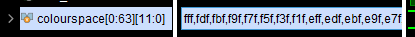
\includegraphics[width=\linewidth]{figures/tb/4.png}
\end{minipage}
This subtractive method appears better, however the aim is to drop the red value by two, whereas here it only drops by one.
The loop in an \lstinline|initial| block does not appear to be synthesised correctly for actual implementation, resulting
in a black screen.

\begin{minipage}{0.475\linewidth}
\begin{lstlisting}[language=Verilog]
for(i=0;i<64;i=i+1)begin
    colourspace[i] = tcol;
    tcol = tcol - 12'h020;
    if(tcol[7:4] < 4'h1) begin
        tcol = tcol - 12'h500;
    end
end 
\end{lstlisting}
\end{minipage}\hfill
\begin{minipage}{0.5\linewidth}
    \centering
    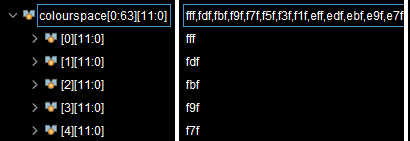
\includegraphics[width=0.9\linewidth]{figures/tb/5.png}
\end{minipage}
The code was moved to an \lstinline|always| block to allow it to be synthesised to the display correctly. 
Furthermore, the reduction was increased. The test bench shows the value stay the same - the 
IF statement is not evaluating true since \lstinline|tcol[7:4]| will move from 1 to F. 

\begin{minipage}{0.475\linewidth}
\begin{lstlisting}[language=Verilog]
for(i=0;i<64;i=i+1)begin
    colourspace[i] = tcol;
    tcol = tcol - 12'h020;
    if(tcol[7:4] == 4'hf) begin
        tcol = tcol - 12'h100;
    end
end 
\end{lstlisting}
\end{minipage}\hfill
\begin{minipage}{0.5\linewidth}
    \centering
    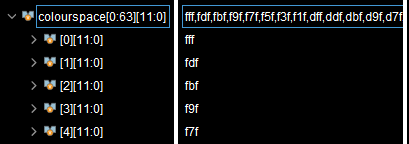
\includegraphics[width=0.9\linewidth]{figures/tb/6.png}
\end{minipage}
The values are now reducing in the correct progression. 